\documentclass{beamer}
\usepackage[romanian]{babel}
\usepackage{ucs}
\usepackage[utf8x]{inputenc}
\PrerenderUnicode{ș}        % Încarcă Unicode ca să scrie ș-ul corect.
\usepackage{relsize}        % Pentru mărimi relative de text.
\usepackage{tikz}           % Pentru diagrame.

% Opțiuni la diagrame tikz.
\usetikzlibrary{patterns, trees, matrix, arrows, decorations.pathmorphing, decorations.pathreplacing}

% Variabile
\newcommand{\autor}{Paul Răzvan Nechifor}
\newcommand{\titlu}{Sistem de fișiere distribuit de tip \eng{peer-to-peer}}
\newcommand{\coordonator}{lector dr. Adrian Iftene}

% Comenzi
\newcommand{\eng}[1]{\emph{#1}} % Pentru cuvinte în limba engleză.
\newcommand{\cod}[1]{\texttt{#1}}
\newcommand{\peers}[3]{
    \def\depl{0.5}
    \def\sep{0.3}
    \def\va{20}
    \def\csep{-\c*\sep-#1}

    \foreach[count=\c] \start/\enda/\endb in {#2} {
        \draw[thick, color=c\c] (\depl+\start-1,\csep) -- (\depl+\enda,\csep);
        \node[plin, color=c\c] at (\depl+\start-1,\csep){};

        \ifnum\endb>0
            \draw[thick, color=c\c] (\depl,\csep) -- (\depl+\endb,\csep);
            \node[plin, color=c\c] at (\depl+\endb,\csep){};
        \else
            \node[plin, color=c\c] at (\depl+\enda,\csep){};
        \fi
    }

    \definecolor{fundal}{rgb}{0.100,0.100,0.400}

    \foreach[count=\c] \v in {#3} {
        \def\vzero{\v0}
        \node[nu, fill=fundal!\vzero] at (\c,-#1-5) {\c};
    }
}

\usetheme{Madrid}
\title{\titlu}
\author{\autor}
\date{3 iulie 2012}

\begin{document}
\definecolor{albastru de fii}{rgb}{0.392, 0.474, 0.737}

% Modific culorile
\setbeamercolor{palette primary}{use=structure,bg=albastru de fii}
\setbeamercolor{palette tertiary}{use=structure,bg=albastru de fii}

% Fără navigation symbols.
\beamertemplatenavigationsymbolsempty

% Modific antetul la diapozitive.
\defbeamertemplate*{footline}{my infolines theme} {
    \leavevmode%
    \hbox{%
    \begin{beamercolorbox}[wd=.2\paperwidth,ht=2.25ex,dp=1ex,center]{author in head/foot}%
        \usebeamerfont{author in head/foot}\insertshortauthor%
    \end{beamercolorbox}%
    \begin{beamercolorbox}[wd=.6\paperwidth,ht=2.25ex,dp=1ex,center]{title in head/foot}%
        \usebeamerfont{title in head/foot}\insertshorttitle%
    \end{beamercolorbox}%
    \begin{beamercolorbox}[wd=.2\paperwidth,ht=2.25ex,dp=1ex,right]{date in head/foot}%
        \usebeamerfont{date in head/foot}\insertshortdate{}\hspace*{2em}%
        \insertframenumber{} / \inserttotalframenumber\hspace*{2ex}%
    \end{beamercolorbox}}%
    \vskip0pt%
}

%%%%%%%%%%%%%%%%%%%%%%%%%%%%%%%%%%%%%%%%%%%%%%%%%%%%%%%%%%%%%%%%%%%%%%%%%%%%%%%%%%%%%%%%%%%%%%%%%%%%%%%%%%%%%%%%%%%%%%%%
\begin{frame}
    \begin{tikzpicture}[overlay]
        \fill[fill=albastru de fii] (-1,-2.8) -- (14,-2.8) -- (14,2) -- (-1,2) -- cycle;
        \node[color=white] at (6, -1.7) {\LARGE \titlu};
    \end{tikzpicture}

    \vspace{4cm}
    \begin{columns}[c]
        \column{4cm}
        % Sigla FII.
        \begin{tikzpicture}[scale=0.36]
            \def\taie{0.5}
            \fill [fill=albastru de fii]
                (0,0) -- (2,0) -- (2,3) -- (3,3) -- (5,5) -- (2,5) -- (2,6) -- (6,6) -- (8,8) -- (0,8) -- cycle;
            \fill [fill=albastru de fii]
                (3,0) -- (3,3-\taie) -- (5,5-\taie) -- (5,0) -- cycle;
            \fill [fill=albastru de fii]
                (6,0) -- (6,6-\taie) -- (8,8-\taie) -- (8,0) -- cycle;
        \end{tikzpicture}
        
        \column{4cm}
        \begin{center}
            {\footnotesize{Absolvent:}}\\
            \autor\\
            \vspace{0.5cm}
            {\footnotesize{Coordonator științific:}}\\
            \coordonator
        \end{center}
    \end{columns}
\end{frame}

%%%%%%%%%%%%%%%%%%%%%%%%%%%%%%%%%%%%%%%%%%%%%%%%%%%%%%%%%%%%%%%%%%%%%%%%%%%%%%%%%%%%%%%%%%%%%%%%%%%%%%%%%%%%%%%%%%%%%%%%
\frame{
    \frametitle{Cuprins}
    \tableofcontents
    Cuvinte cheie: sistem de fișiere, partajare de fișiere, \eng{peer-to-peer}, organizare
}

%%%%%%%%%%%%%%%%%%%%%%%%%%%%%%%%%%%%%%%%%%%%%%%%%%%%%%%%%%%%%%%%%%%%%%%%%%%%%%%%%%%%%%%%%%%%%%%%%%%%%%%%%%%%%%%%%%%%%%%%
\section{Motivație}
\begin{frame}{Motivație}
    Am ales această temă deoarece am observat o serie de îmbunătățiri care pot fi aduse metodelor de partajare curente.
    \\~\\
    Probleme:
    \begin{itemize}
        \item organizarea într-o ierarhie centrală
        \item permanența în rețea
        \item modificări ulterioare
        \item accesul aleator la fișiere
        \item gradul de control al creatorilor
    \end{itemize}
    ~\\
    Inspirație:
    \begin{itemize}
        \item servere BitTorrent private
        \item sisteme de fișiere P2P existente (Ivy, Pastis)
    \end{itemize}
\end{frame}

%%%%%%%%%%%%%%%%%%%%%%%%%%%%%%%%%%%%%%%%%%%%%%%%%%%%%%%%%%%%%%%%%%%%%%%%%%%%%%%%%%%%%%%%%%%%%%%%%%%%%%%%%%%%%%%%%%%%%%%%
\section{Funcționarea protocolului}
\begin{frame}{Funcționarea protocolului}
    \begin{itemize}
        \item o autoritate care decide
        \item un utilizator alege un număr de blocuri pe care să le rețină
        \item serverul decide alocarea blocurilor (se pot acorda priorități)
        \item un client descarcă blocurile alocate lui și le încarcă la cerere
        \item serverul semnează operațiile de modificare a sistemului de fișiere
    \end{itemize}

    % Setez unitățile în pt ca să aliniez mai ușor nodurile.
    \begin{center}
        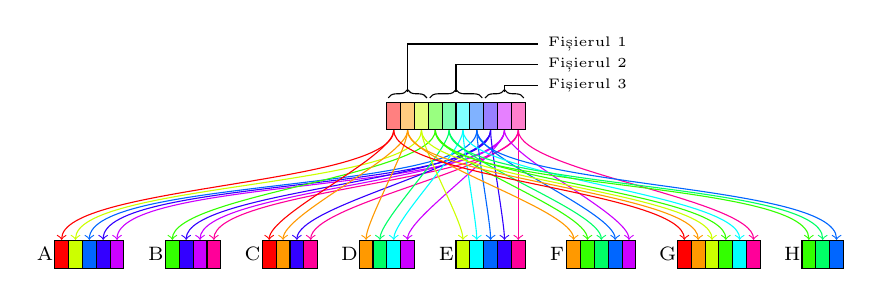
\begin{tikzpicture}[x=5pt, y=5pt]
            \tikzstyle{nod}  = [draw, inner sep=0pt, minimum height=10pt, minimum width=5pt]
            \tikzstyle{tran} = [->]%, >=latex]

            \definecolor{c1}{rgb}{1.000,0.000,0.000}
            \definecolor{c2}{rgb}{1.000,0.600,0.000}
            \definecolor{c3}{rgb}{0.800,1.000,0.000}
            \definecolor{c4}{rgb}{0.200,1.000,0.000}
            \definecolor{c5}{rgb}{0.000,1.000,0.400}
            \definecolor{c6}{rgb}{0.000,1.000,1.000}
            \definecolor{c7}{rgb}{0.000,0.400,1.000}
            \definecolor{c8}{rgb}{0.200,0.000,1.000}
            \definecolor{c9}{rgb}{0.800,0.000,1.000}
            \definecolor{c10}{rgb}{1.000,0.000,0.600}

            % Desenează sistemul complet.
            \foreach \c in {1,...,10}
                \node[nod, fill=c\c!50] (sis\c) at (0+\c, 0) {};

            % Desenează acoladele cu explicațiile
            \tikzstyle{acol} = [decorate, decoration={brace, amplitude=3pt, raise=1.5pt}]
            \tikzstyle{fis} = [font=\tiny]
            \def\desubt{1.0}
            \def\sp{0.1} % spatiere
            \draw[acol] (0.5+\sp,\desubt) -- ( 3.5-\sp,\desubt) node[midway] (f1a) {};
            \draw[acol] (3.5+\sp,\desubt) -- ( 7.5-\sp,\desubt) node[midway] (f2a) {};
            \draw[acol] (7.5+\sp,\desubt) -- (10.5-\sp,\desubt) node[midway] (f3a) {};
            \node[fis] (f1t) at (15, 5.2) {Fișierul 1};
            \node[fis] (f2t) at (15, 3.7) {Fișierul 2};
            \node[fis] (f3t) at (15, 2.2) {Fișierul 3};
            \draw (f1a) |- (f1t);
            \draw (f2a) |- (f2t);
            \draw (f3a) |- (f3t);

            % Desenează partenerii.
            \foreach \x/\y/\cod/\na/\nb/\nc/\nd/\ne/\nf/\ng/\nh in {
                     -24/-10/A/1/3/7/8/9/0/0/0,
                     -16/-10/B/4/8/9/10/0/0/0/0,
                      -9/-10/C/1/2/8/10/0/0/0/0,
                      -2/-10/D/2/5/6/9/0/0/0/0,
                       5/-10/E/3/6/7/8/10/0/0/0,
                      13/-10/F/2/4/5/7/9/0/0/0,
                      21/-10/G/1/2/3/4/6/10/0/0,
                      30/-10/H/4/5/7/0/0/0/0/0
            } {
                \node (\cod) at (\x-0.2,\y) {\scriptsize \cod};
                \foreach[count=\c] \cul in {\na,\nb,\nc,\nd,\ne,\nf,\ng,\nh} {
                    \ifnum\cul>0
                        \node[nod, fill=c\cul] (\cod\c) at (\x+\c,\y){};
                        \draw[tran, color=c\cul] (sis\cul) edge[out=-90, in=90, looseness=0.4] (\cod\c);
                    \fi
                }
            }

        \end{tikzpicture}
    \end{center}
\end{frame}

%%%%%%%%%%%%%%%%%%%%%%%%%%%%%%%%%%%%%%%%%%%%%%%%%%%%%%%%%%%%%%%%%%%%%%%%%%%%%%%%%%%%%%%%%%%%%%%%%%%%%%%%%%%%%%%%%%%%%%%%
\section{Vizualizarea sistemului de fișiere}
\begin{frame}{Vizualizarea sistemului de fișiere}
    \begin{center}
        \begin{tikzpicture}[x=5pt, y=5pt]
            \tikzstyle{cale}  = [font=\tiny, inner sep=0pt, minimum height=0.7cm, minimum width=11.1cm,
                    fill=albastru de fii!60]
            \tikzstyle{descriere}  = [font=\tiny, fill=albastru de fii, text=white]
            \node[cale] (Z) at (0,10) {Partener 1, 2, ...};
            \node[cale] (A) at (0,0) {\texttt{/filme opensource/film 1.mkv}};
            \node[cale] (B) at (0,-10) {\texttt{ftp://127.0.0.1:3000/filme opensource/film 1.mkv}};
            \node[cale, minimum width=5.5cm] (C1) at (-16,-20) {\texttt{/media/negura/filme opensource/film 1.mkv}};
            \node[cale, minimum width=5.5cm] (C2) at (16,-20) {\texttt{U:\textbackslash{}filme opensource\textbackslash{}film 1.mkv}};

            \foreach \x/\y/\textul in {
                    0/7.5/descărcare,
                    0/-2.5/server FTP local pe portul 3000,
                    -16/-12.5/montare Unix în \texttt{/media/negura},
                    16/-12.5/montare Windows în unitatea \texttt{U:}
            } {
                \def\w{0.5}
                \def\h{4}
                \def\e{0.5}
                \fill[fill=albastru de fii] (\x-\w,\y) -- (\x+\w,\y) -- (\x+\w,\y-\h) -- (\x+\w+\e,\y-\h) 
                -- (\x,\y-\h-\w-\e) -- (\x-\w-\e,\y-\h) -- (\x-\w,\y-\h) -- cycle;
                \node[descriere] at (\x,\y-2) {\textul};
            }
        \end{tikzpicture}
    \end{center}
\end{frame}

%%%%%%%%%%%%%%%%%%%%%%%%%%%%%%%%%%%%%%%%%%%%%%%%%%%%%%%%%%%%%%%%%%%%%%%%%%%%%%%%%%%%%%%%%%%%%%%%%%%%%%%%%%%%%%%%%%%%%%%%
\section{O îmbunătățire}
\begin{frame}{O îmbunătățire}
    Lista de blocuri se modifică dinamic și este definită de doi parametrii: numărul total de blocuri și poziția de
    început.\\~\\

    \begin{center}
        % Setez unitățile în pt ca să aliniez mai ușor nodurile.
        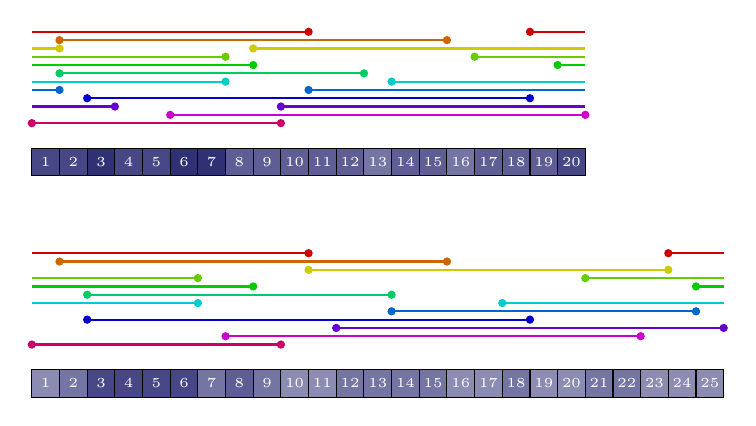
\begin{tikzpicture}[x=10pt, y=10pt]
            \tikzstyle{every node} = [font=\tiny, text=white]
            \tikzstyle{nu}  = [draw, inner sep=0pt, minimum height=10pt, minimum width=10pt]
            \tikzstyle{plin}  = [fill, circle, inner sep=0pt, minimum height=3pt, minimum width=3pt]
            \tikzstyle{textul} = [node distance=1.6cm, inner sep=0pt, anchor=west, text width=2.6cm]

            \definecolor{c1}{rgb}{0.800,0.000,0.000}
            \definecolor{c2}{rgb}{0.800,0.400,0.000}
            \definecolor{c3}{rgb}{0.800,0.800,0.000}
            \definecolor{c4}{rgb}{0.400,0.800,0.000}
            \definecolor{c5}{rgb}{0.000,0.800,0.000}
            \definecolor{c6}{rgb}{0.000,0.800,0.400}
            \definecolor{c7}{rgb}{0.000,0.800,0.800}
            \definecolor{c8}{rgb}{0.000,0.400,0.800}
            \definecolor{c9}{rgb}{0.000,0.000,0.800}
            \definecolor{c10}{rgb}{0.400,0.000,0.800}
            \definecolor{c11}{rgb}{0.800,0.000,0.800}
            \definecolor{c12}{rgb}{0.800,0.000,0.400}

            \peers{0}{19/20/10,2/15/0,9/20/1,17/20/7,20/20/8,2/12/0,14/20/7,11/20/1,3/18/0,10/20/3,6/20/0,1/9/0}
                    {8,8,9,8,8,9,9,7,7,7,7,7,6,7,7,6,7,7,7,8}
            \peers{8}{24/25/10,2/15/0,11/23/0,21/25/6,25/25/8,3/13/0,18/25/6,14/24/0,3/18/0,12/25/0,8/22/0,1/9/0}
                    {5,6,8,8,8,8,6,7,6,5,5,6,6,6,6,5,5,6,5,5,6,6,5,5,5}
        \end{tikzpicture}
    \end{center}
\end{frame}

%%%%%%%%%%%%%%%%%%%%%%%%%%%%%%%%%%%%%%%%%%%%%%%%%%%%%%%%%%%%%%%%%%%%%%%%%%%%%%%%%%%%%%%%%%%%%%%%%%%%%%%%%%%%%%%%%%%%%%%%
\section{Concluzii}
\begin{frame}{Concluzii}
    O soluție pentru rețele metropolitane. Motive:
    \begin{itemize}
        \item pentru fluxare este nevoie de viteze mari între parteneri
        \item fiind nevoie de un server central rețeaua nu poate fi foarte mare
    \end{itemize}
    Utilitate: adunarea într-un grup a unor fișiere care au o anumită specializare sau temă.
\end{frame}

%%%%%%%%%%%%%%%%%%%%%%%%%%%%%%%%%%%%%%%%%%%%%%%%%%%%%%%%%%%%%%%%%%%%%%%%%%%%%%%%%%%%%%%%%%%%%%%%%%%%%%%%%%%%%%%%%%%%%%%%
\section{Demonstrație}
\begin{frame}{Demonstrație}
    \begin{center}
        ...funcționarea aplicațiilor...
    \end{center}
\end{frame}

\end{document}
